\section{Idee}
Das Genre des Tower Defense Spiele ist sehr verbreitet. Die meisten dieser Spiele sind webbasiert und mit Flash realisiert. Ziel diese Projektes ist es ein Javabasiertes multiplayer Tower Defense zu realisieren.

Das Spiel wird im Internet zum Download angeboten \colorbox{yellow}{(gratis / kostenpflichtig)}, sodass es sich auf dem Markt verbreiten kann.

Der grosse Unterschied zu anderen Tower Defense Spielen ist die Wichtigkeit der Zusammenarbeit der beteiligten Spieler:
\begin{itemize}
 \item Einzelne Türme werden zu teuer sein, sodass man diese nicht ohne Hilfe der anderen Spieler kaufen kann.
 \item Die Spieler haben die Möglichkeit, einen Tower von einem anderen Spieler zu upgraden. Diese Upgrades stehen für die eigenen Towers nicht zur Verfügung.
 \item Es besteht die Möglichkeit, dass die Spieler sich Geld zur Unterstützung einander überweisen.
\end{itemize}

\begin{figure}[htb]
 \begin{center}
  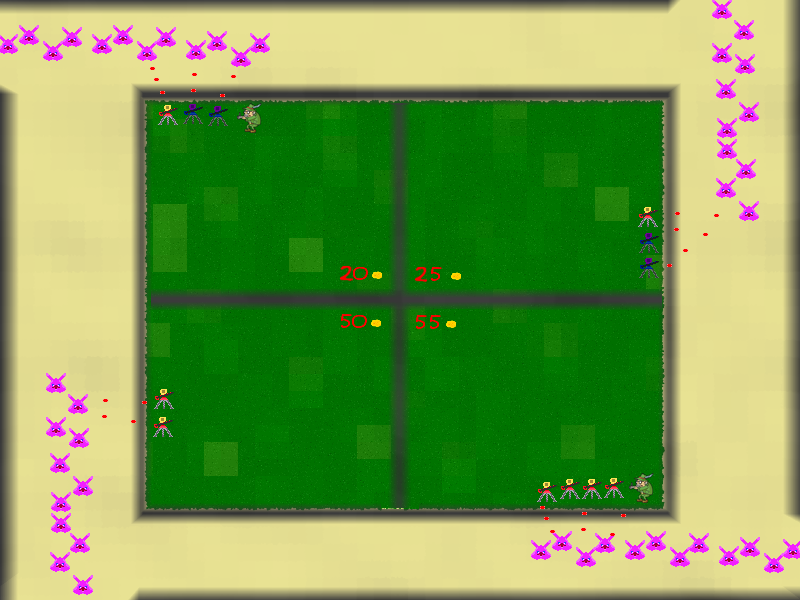
\includegraphics[scale=0.7]{spielfeld}
 \end{center}
 \caption{Skizze des Spielfelds}
 \label{fig:spielfeld_skizze}
\end{figure}

\subsection{Begriffserkährung Tower Defense}
Tower Defense Spiele basieren immer auf dem selben Grundprinzip:
Es existieren 4 Hauptelemente. Die Karte(Bauplatz für Spieler), Der Weg, die Gegner und die Türme.
Die Gegner laufen dem vordefinierten Weg entlang und der Spieler kann Türme bauen (meistens verschiedene Typen), welche autonom auf die Gegner schiessen, worauf die Gegner Lebenspunkte verlieren.
